\chapter{Objetivos}\label{cap.objetivos}
Una vez explicado el contexto de este proyecto, se describirán los objetivos, los requisitos y la metodología que se han empleado.\\

El propósito principal de este proyecto es la creación o mejora de tres prácticas para el entorno docente JdeRobot-Academy. En concreto una práctica de navegación global, una práctica de una aspiradora robótica y, por último, una práctica acerca del aparcamiento de coches autónomos. Siguiendo el diseño de JdeRobot-Academy, para cada práctica hay que crear 4 ingredientes:

\begin{itemize}
\item Enunciado e infraestructura en simulador
\item Componente académico que incluye \acrshort{gui}
\item Solución tentativa
\item Evaluador automático
\end{itemize}

\section{Objetivos}
El objetivo principal de este proyecto es la creación de prácticas para el entorno JdeRobot-Academy, el cual emplearán los alumnos. En cada una de estas prácticas se elaborará toda la infraestructura que se comunica con el Simulador Gazebo, donde el alumno podrá ver el resultado de la ejecución de su algoritmo. Todos los robots que se emplean en las prácticas son simulados. Además, se creará el entorno gráfico que facilitará al alumno la resolución de las prácticas; así como un evaluador automático que mide diferentes parámetros de cada práctica y permite la corrección de cada una de ellas en función de dichos parámetros. Para cada una de las prácticas se ofrece una posible solución. Se ofrecerá, en cada práctica, un fichero MyAlgorithm.py donde el alumno podrá programar su solución.\\

En este proyecto, como hemos mencionado antes, se llevarán a cabo tres prácticas. Para cada una de estas prácticas se han creado todos los elementos mencionados en el párrafo anterior. Lo que difiere en estas prácticas es el escenario de cada una de ellas, los diferentes elementos que se mostrarán en el interfaz gráfico, los elementos que tendrá en cuenta el evaluador automático a la hora de calcular la nota de cada alumno, y por último el algoritmo de la solución.\\

En la práctica ``TeleTaxi'' el objetivo es que el alumno aprenda técnicas de navegación global, en concreto, la técnica Gradient Path Planning. Está práctica no es totalmente original, sino que existía una versión previa de la infraestructura y del componente académico, pero presentaban ciertos problemas. Por ello, en este proyecto se va a mejorar tanto la infraestructura como el componente académico, así como se va a desarrollar una solución de referencia y un evaluador automático que nos permita calificarla.\\

En la práctica ``Aspiradora Autónoma'' el principal objetivo es que el alumno sea capaz de proporcionar una solución para la limpieza de una casa sin autolocalización. En concreto, este algoritmo se basará en el algoritmo que llevan a cabo los modelos de la serie 500 de Roomba de iRobot. Se realizará una solución que limpia en función de tres modos de limpieza: giro en espiral, seguimiento de paredes y cruce de habitación. La aspiradora cuenta con diferentes sensores y actuadores, entre los que se encuentran un sensor láser, sensores de posición, un sensor bumper, y actuadores que permiten dar órdenes a la aspiradora de velocidad de tracción y velocidad de giro.  En este caso la práctica se ha realizado desde cero, pues no existía una versión previa. Con ella los alumnos se familiarizarán con un problema robótico real, cotidiano y que ya se está comercializando.\\


En último lugar, en la práctica ``Aparcamiento Automático'', el propósito es la realización de una solución que sea capaz de aparcar un coche de forma autónoma. El taxi está dotado de tres sensores láser (que se encuentran en la parte frontal, en la parte trasera y en el lateral derecho) para poder medir distancias a los coches y encontrar aparcamiento. La solución propuesta es una solución ``ad hoc'' mediante un algoritmo basado en las medidas sensoriales que se obtienen de los lásers. La solución permite al taxi encontrar una plaza de aparcamiento libre y realizar la maniobra de aparcamiento. Esta práctica, la cual ha sido realizada de cero, nos permitirá acercarnos a problemas robóticos que ya existen en el mercado (Volkswagen, Tiguan, etc) y con ello aprender cómo funcionan.

\section{Requisitos}
El desarrollo del proyecto estará guiado por los objetivos mencionados anteriormente y deberá ajustarse a los requisitos de partida del proyecto, los cuales hacen que la solución esté condicionada. Estos requisitos son:

\begin{enumerate}[1.]
\item En este proyecto todas las simulaciones se realizarán en el simulador Gazebo, en concreto en la versión 7. Los modelos de robots que se emplearán serán creados. En este caso se utilizarán dos taxis (los cuales tienen diferentes sensores) y el modelo Roomba.
\item Se hará uso de la plataforma JdeRobot en su versión 5.5.2, que se explicará con detalle en el siguiente capítulo~\ref{cap.infraestructura}. El uso de esta plataforma simplifica el desarrollo del comportamiento del robot. 
\item El sistema operativo que se empleará para este proyecto será Ubuntu 16.04.
\item El lenguaje de desarrollo empleado para crear los plugins necesarios será C++. Sin embargo, en el resto de componentes se utilizará el lenguaje Python 2. Este requisito restringe la solución a que se programe en Python 2.
\item Las soluciones han de ser vivaces. Los algoritmos propuestos no pueden detenerse mucho tiempo a pensar cuál será el próximo movimiento del robot, porque han de reaccionar rápido, en tiempo real y con movimientos suaves.
\end{enumerate}

\section{Metodología}
El proyecto se ha basado en una metodología iterativa, donde cada iteración se compone de varias fases: determinar objetivos, planificación, diseño e implementación, análisis de riesgos, así como reuniones periódicas con el tutor.\\

Para desarrollar este proyecto se ha optado por seguir el modelo de desarrollo en espiral, creado por Barry Boehm. Este modelo se adapta perfectamente a este tipo de proyectos, ya que permite separar el comportamiento final en varias subtareas más sencillas para después juntarlas. Este modelo permite una gran flexibilidad ante cambios en los requisitos, algo bastante común en el desarrollo de proyectos.\\

Este modelo de ciclo de vida permite ir obteniendo prototipos funcionales, a la vez que se realiza el desarrollo del producto de forma incremental. El modelo consta de iteraciones, que se pueden llamar ciclos. En cada ciclo existen cuatro fases bien diferenciadas:

\begin{itemize}
\item Determinar o fijar objetivos: En esta fase se definen los objetivos específicos que deben cumplirse para que el ciclo actual pueda considerarse finalizado en base a los objetivos finales. Conforme vayan sucediéndose más iteraciones, los objetivos serán más complejos.
\item Análisis del riesgo: En esta fase se efectúa un análisis detallado para cada uno de los riesgos que pueda tener el objetivo fijado en la fase anterior. Se definen los pasos a seguir para minimizar los riesgos y después del análisis se planean estrategias alternativas.
\item Desarrollar y probar: En la tercera fase, se desarrolla el producto o las partes del producto que se han acordado en las fases anteriores. Además, se llevarán a cabo las pruebas oportunas que nos permitan asegurar la calidad de la implementación, y que pueda seguir sirviendo en iteraciones futuras.
\item Planificación: En esta última fase, es donde se revisan los resultados obtenidos mediante las pruebas de la fase anterior, y es donde se planifica la iteración siguiente teniendo en cuenta los posibles errores que se han cometido.
\end{itemize}

\begin{figure}[H]
  \begin{center}
    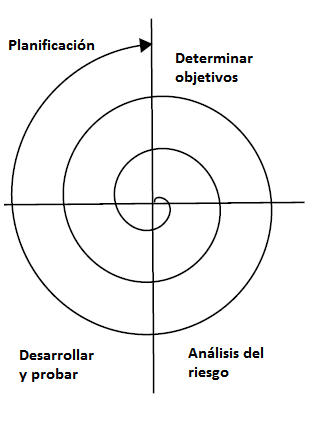
\includegraphics[width=0.4\textwidth]{figures/Objetivos/espiral.png}
		\caption{Modelo en espiral}
		\label{fig.espiral}
		\end{center}
\end{figure}

Para poder llevar a cabo esta metodología se han mantenido reuniones semanales con el tutor. En estas reuniones se analizaban los resultados de cada iteración, y en función de los resultados se fijaban nuevos objetivos y se planteaban posibles vías para resolverlos. El código que se ha ido desarrollando semanalmente se ha subido al repositorio propio público de Github \footnote{\url{https://github.com/RoboticsURJC-students/2016-tfg-vanessa-fernandez}}, que emplea el sistema de control de versiones. Además, las tareas realizadas se han ido mostrando semanalmente mediante explicaciones, vídeos o imágenes en la bitácora de la página de JdeRobot \footnote{\url{http://jderobot.org/Vmartinezf-tfg}} y  han sido integradas en el repositorio oficial de JdeRobot-Academy.

\section{Plan de trabajo}
En esta sección se exponen las etapas temporales en las que se ha dividido el proyecto, que además se corresponden con el modelo en espiral:

\begin{itemize}
\item Familiarización con el entorno JdeRobot y OpenCV. En esta etapa se ha descargado e instalado la plataforma JdeRobot, el entorno docente JdeRobot-Academy, y todo el software necesario para el desarrollo del proyecto. En esta fase se engloba el aprendizaje del uso de Github, para el control de versiones, y el aprendizaje básico de la librería OpenCV. Para poder cerrar esta fase se han realizado algunas soluciones de prácticas existentes del entorno JdeRobot-Academy.
\item Familiarización con el simulador Gazebo y sus plugins. En esta etapa se ha estudiado código de la plataforma JdeRobot, así como el material disponible en Gazebo en la página oficial \footnote{\url{http://gazebosim.org/}}.  Además, se han realizado pruebas creando mundos simples en Gazebo mediante modelos ya disponibles. También se ha realizado un estudio de los plugins creados en JdeRobot (compilación e instalación), aprendizaje básico de C++, y desarrollo de algún plugin necesario para el desarrollo de las prácticas.
\item Desarrollo de la práctica ``TeleTaxi''. La creación de esta práctica implica el desarrollo del mundo y modelos necesarios para dicha práctica. Con dichos modelos se ha podido crear el mundo que será empleado en esta práctica. Posteriormente, se ha llevado a cabo el desarrollo de la interfaz gráfica que facilita la resolución de la práctica a los alumnos. Para ello ha sido necesario antes familiarizarse con la herramienta PyQt5. El siguiente paso que se ha abordado es el desarrollo del evaluador automático que permitirá calificar la práctica. Este evaluador automático se ha creado mediante la utilización de PyQt5. Por último, se ha llevado a cabo el desarrollo de la solución, lo que implica la programación de la planificación más la programación del pilotaje del robot.
\item Desarrollo de la práctica ``Aspiradora Autónoma''. En esta etapa ha sido necesario desarrollar inicialmente los modelos necesarios para la práctica, los cuales han permitido crear el entorno (mundo de Gazebo) de la práctica. El siguiente paso ha sido el desarrollo del componente académico (interfaz gráfica) que permite a los alumnos realizar la solución de una manera más sencilla. A continuación, se ha desarrollado el evaluador automático que permitirá evaluar la práctica. Finalmente, se ha desarrollado la solución, en la cual se realizará el pilotaje del robot en base a una planificación y los datos proporcionados por los sensores.
\item Desarrollo de la práctica ``Aparcamiento automático''. Al igual que en las prácticas anteriores ha sido necesario abordar diferentes etapas para el desarrollo de la práctica. Inicialmente, se han creado los modelos que se emplean en la práctica, así como el escenario que incluye estos modelos. Posteriormente, se ha desarrollado el componente académico que ayudará a los alumnos a conocer distintos factores que influyen al resolver la práctica. A continuación, se ha abordado la creación del evaluador automático que calificará la práctica. Finalmente, se ha realizado la solución de la práctica, la cual implica realizar el pilotaje del robot basándose en los datos proporcionados por los sensores.
\end{itemize}